\documentclass{article}
\usepackage{tikz}
\usetikzlibrary{arrows}
\usepackage[english]{babel}
\usepackage[utf8]{inputenc}
\usepackage{minted}
\usepackage{fancyhdr}
\usepackage{graphicx}
\usepackage{amsmath}
\usepackage[margin=1in]{geometry}

\addtolength{\topmargin}{.2in}
\graphicspath{{./queue_lengths/}}
 
\pagestyle{fancy}
\fancyhf{}
\rhead{Austin Bursey , Aaron Exley\\ Tim McGill, Joseph Myc}
\lhead{CP468 A2\\November 11th 2019}
\rfoot{Page \thepage}
\begin{document}

\begin{titlepage}
  \pagestyle{fancy}
  \thispagestyle{fancy}
   \begin{center}
       \vspace*{1cm}
 
      \Huge
       \textbf{Assignment 2}
 
       \vspace{0.5cm}
       \Large
        CP468 \\ November 11th 2019
 
       \vspace{1.5cm}
 
       \textbf{Austin Bursey , Aaron Exley, Tim McGill, Joseph Myc}
 
       \vfill

       \vspace{0.8cm}
 
   \end{center}
\end{titlepage}
\setcounter{page}{2}

\section{Binary Constraints}
The binary version of the constraints for the csp is that every cell in the puzzle, has the constraint where its value can not be equal to any of its neighbours  values. This results in 8 constraints for the row neighbours, 8 constraints for the column neighbours, and 8 constraints for the box neighbours. This results in 24 constraints for each node in the puzzle, so across the 81 node there are a total of 1944 constraints.\\
\newline
A more mathematical way to represent the constraints for each cell  in the Sudoku is as follows:\\
For the Rows:
\begin{align*}
cell[x, y].value \ne cell[i, y].value,\quad i=0\rightarrow8\,and\, i \ne x
\end{align*}
For the Columns:
\begin{align*}
cell[x, y].value \ne cell[x, j].value,\quad j=0\rightarrow8\,and\, j \ne y
\end{align*}
For the Box's:
\begin{align*}
cell[x, y].value \ne cell[i, j].value,\quad i=[x-(x\%3)]\rightarrow[x+(2-(x\%3))]\,and\, i \ne x \\
												j=[y-(y\%3)]\rightarrow[y+(2-(y\%3))]\, and\, j \ne y
\end{align*}
\section{AC3 Queue Size}

The length of the queue was recorded after every iteration of the AC3 algorithm, and then plotted on a graph.
\newline
In the case where the Sudoku was solved with AC3 alone we get a graph that looks as follows

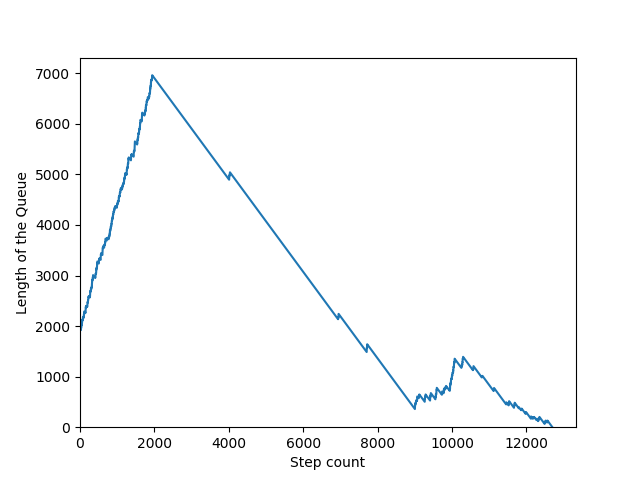
\includegraphics[scale=0.6]{Sudoku-Queue-length-plot-29}

In the case where the Sudoku was not solved with AC3, backtracking is used. In the backtracking algorithm AC3 is called after every assignment to make sure the csp is still arc consistent with that assignment. We still kept track of the length for every call, every time the graph reaches 0 is when an AC3 call finishes.

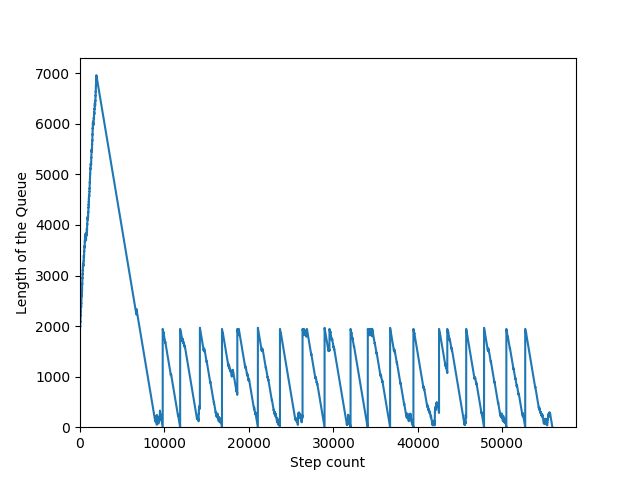
\includegraphics[scale=0.6]{Sudoku-Queue-length-plot-10}

\section{Input format}

For the input we decided to go with a string read from a file that is 81 characters long with a . as the placeholder for empty cells.\\
\newline
Here is an example of one of the inputs:
\newline
\begin{verbatim}
.........27.....14....8.573...745186.....2......8....7.485.......647..2..1....6..
\end{verbatim}
Is equal to the puzzle:
\begin{verbatim}
-------------------------
| . . . | . . . | . . . |
| 2 7 . | . . . | . 1 4 |
| . . . | . 8 . | 5 7 3 |
-------------------------
| . . . | 7 4 5 | 1 8 6 |
| . . . | . . 2 | . . . |
| . . . | 8 . . | . . 7 |
-------------------------
| . 4 8 | 5 . . | . . . |
| . . 6 | 4 7 . | . 2 . |
| . 1 . | . . . | 6 . . |
-------------------------
\end{verbatim}

\newpage
\section{Implementation of AC3 (with backtracking) for Sudoku }
\begin{minted}{python}

from queue import Queue
from copy import deepcopy
import sys
import os
#for the graph at the end
import matplotlib.pyplot as plt

class Node:
    def __init__(self,row,col,value=None, domain=range(1, 10)):
        self.row = row
        self.col = col
        if value is not None: 
            self.value = int(value)
            self.domain = [int(value)]
        else : 
            self.value = value
            self.domain = list(domain)
        
    def __str__(self):
        return '({}, {}, {}, {})'.format(self.row, self.col, self.value, self.domain)

    def __repr__(self):
        return '({}, {}, {}, {})'.format(self.row, self.col, self.value, self.domain)

class Arc: 
    def __init__(self,Xi,Xj):
        self.Xi = Xi
        self.Xj = Xj 

    def evaluate(self):
        '''
        Evaluates arc
        ---------------------------
        returns:
            noSolution: whether or not the state of the puzzle is not solvable
            Checks : Xi != Xj and Xi domain not {}
        '''
        notSolvable = False 
        #enforcing arc consistency Xi != Xj 
        if(self.Xi.value is not None and self.Xi.value == self.Xj.value):
            notSolvable = True 
        elif (self.Xj.value != None and self.Xj.value in self.Xi.domain):
            self.Xi.domain.remove((self.Xj.value))
            if (len(self.Xi.domain)< 0 ): 
                notSolvable = True
        return notSolvable
\end{minted}
\newpage
\begin{minted}{python}
def addNeighbours(queue,node, puzzle):
    '''
    Adds all Arcs where Xk != Xi given Xi. 
    ---------------------------
    Params:
        queue: a Queue of of arcs to evaluate using AC3
        node: the node Xi you would like to add all neighbhor arcs to
        puzzle: a 2d array of Nodes representing the puzzle
    returns:
        puzzle: a 2d array of Nodes representing the puzzle
        noSolution: a boolean of whether or not the given puzzle is solvable
        noneValueFound: a boolean of whether the given puzzle was fully solved by AC3, 
        returns true if AC3 solved the puzzle
    '''
    currentRow = node.row
    currentColumn = node.col
    #grab neighbhors in nodes row
    i = currentRow
    for j in range(9): 
        if not (currentRow == i and currentColumn == j):
            queue.put(Arc(puzzle[i][j], node ))

    #grab neighbhors in nodes column
    j = currentColumn
    for i in range(9): 
        if not (currentRow == i and currentColumn == j):
            queue.put(Arc(puzzle[i][j], node ))

    #grab neighbhors in box
    row = (currentRow // 3) * 3
    col = (currentColumn // 3) * 3

    for i in range(3) :
        for j in range(3) :
            if not (currentRow == row +i and currentColumn == col+ j):
                queue.put(Arc(puzzle[row + i][col + j], node ))

def AC3(puzzle): 
    '''
    Does AC3 algorithm on Sudoku Puzzle
    ---------------------------
    Params:
        puzzle: a 2d array of Nodes representing the puzzle
    returns:
        puzzle: a 2d array of Nodes representing the puzzle
        noSolution: a boolean of whether or not the given puzzle is solvable
        noneValueFound: a boolean of whether the given puzzle was fully solved by AC3,
        returns true if AC3 solved the puzzle
    '''
    global qlengths
    queue = Queue()
\end{minted}
\newpage
\begin{minted}{python}
    #fill queue with initial constraints
    for row in puzzle:
        for node in row: 
            currentRow = node.row
            currentColumn = node.col
            #grab neighbhors in nodes row
            i = currentRow
            for j in range(9): 
                if not (currentRow == i and currentColumn == j):
                    queue.put(Arc(node,puzzle[i][j] ))

            #grab neighbhors in nodes column
            j = currentColumn
            for i in range(9): 
                if not (currentRow == i and currentColumn == j):
                    queue.put(Arc( node,puzzle[i][j] ))

            #grab neighbhors in box
            num_row = (currentRow // 3) * 3
            col = (currentColumn // 3) * 3

            for i in range(3) :
                for j in range(3) :
                    if not (currentRow == num_row +i and currentColumn == col+ j):
                        queue.put(Arc(node,puzzle[num_row+ i][col+j] ))
                        
    noSolution = False
    qlengths.append(queue.qsize())
    while (queue.qsize() >  0  and not noSolution): 
        #Get first Node
        arc = queue.get_nowait()
        node = arc.Xi
        
        #get needed attributes
        domainCount = len(node.domain)
        noSolution= arc.evaluate()
        newDomainCount = len(node.domain)

        # this line doesnt cause a problem due to the check within "evaluate"
        # because of this line : if(self.Xi.value is not None and 
        # self.Xi.value == self.Xj.value):
        if newDomainCount == 1 :
            node.value = node.domain[0]
        #if domain has been changed , add all neighbors
        if newDomainCount < domainCount:
            addNeighbours(queue,node,puzzle)
        qlengths.append(queue.qsize())
\end{minted}
\newpage
\begin{minted}{python}
    i=0 
    j= 0 
    #checking if puzzle is solved
    noneValueFound= False
    while (i < 9 and not noneValueFound):
        j = 0
        while(j < 9 and not noneValueFound):
            if puzzle[i][j].value is None: 
                noneValueFound = True
            j+=1
        i +=1 
    return puzzle, not noneValueFound, noSolution

def loadPuzzle(file='./puzzles/easy.csv', num=1, header=True, start=0, 
                givenSolutions=False):
    '''
    Loads a puzzle from a file
    ---------------------------
    Params (optional):
        file: the file to load, defaults to puzzle/easy.csv
        num: the number of puzzles to load, defaults to 1
        header: if the file has a header or not, defaults to True
        start: what line to start reading the puzzle from
    returns:
        puzzle: a 2d array of Nodes representing the puzzle
        solution: a 2d array of Nodes representing the solution of the puzzle
        Note: if num > 1 will return an array of puzzles and and array of solutions
    '''
    with open(file, 'r') as f:
        
        if num == -1 or num > 1:
            puzzles = []
            solutions = []

        for i, line in enumerate(f):
            if header and i == 0:
                start += 1
                continue

            if i < start:
                continue
        
            if num != -1 and i > start + num:
                break
            
            if givenSolutions:
                puzzleAndSol = line.split(',')
            else:
                line = line.replace(',', '')
                puzzleAndSol = [line]
            puzzle = []
            for j in range(9):
                row = []
                for k in range(9):
                    row.append(Node(j, k, 
                    None if puzzleAndSol[0][j*(9) + k] == '.' else 
                            puzzleAndSol[0][j*(9) + k]))
                puzzle.append(row)

            if givenSolutions:
                solution = []
                for j in range(9):
                    row = []
                    for k in range(9):
                        row.append(Node(j, k, 
                        None if puzzleAndSol[1][j*(9) + k] == '.' else 
                                puzzleAndSol[1][j*(9) + k]))
                    solution.append(row)

            if num == -1 or num > 1:
                puzzles.append(puzzle)
                if givenSolutions:
                    solutions.append(solution)
    if num == -1 or num > 1:
        return puzzles, solutions
    else:
        return puzzle, solution if givenSolutions else None

def backtrackSearch(puzzle):
    '''
    Performs a backtracking search on a csp sudoku
    ---------------------------
    Param:
        puzzle: A 2d array of Node objects
    returns:
        A solved sudoku puzzle
        A boolean of if the puzzle is solved or not
    '''

    # Find the starting node based on the degree heuristic
    # ie selecting the node with largest amount of constraints
    # since that node will have the largest degree as there will
    # be the most unassigned variables around it.
    firstNode = None
    for row in puzzle:
        for node in row:
            if node.value is None and (firstNode is None 
            or len(firstNode.domain) < len(node.domain)):
                firstNode = node

    # Starts the backtracking
    return backtrack(puzzle, firstNode.row, firstNode.col)
\end{minted}
\newpage
\begin{minted}{python}
def backtrack(puzzle, row, col):
    '''
    Auxiliary Performs a backtracking search on a csp sudoku
    ---------------------------
    Params:
        puzzle: A 2d array of Node objects
        row: The row of the current node
        col: The col of the current node
    returns:
        A solved sudoku puzzle
        A boolean for if the puzzle is solved or not
    '''
    
    # Check if the puzzle is finished, if it is we are done
    # and collapse the call stack
    if complete(puzzle):
        return puzzle, True

    # Get the order of the domain using the
    # least consraining value heuristic
    domainOrder = order(row, col, puzzle)

    for value in domainOrder:

        # Check if the current value in the domain is consistant
        # with the constraints of the sudoku
        # Should always be consisitant
        if valid(puzzle, row, col, value):

            # Store a copy of the current state for
            # the backtracking
            state = deepcopy(puzzle)

            # Update the value of the current node
            puzzle[row][col].value = value

            # Make the updated puzzle arc consistant
            puzzle, completed, noSolution = AC3(puzzle)

            # If the puzzle still has a solution
            # We can continue, Otherwise we move on 
            if not noSolution:
                if not completed:
                    # Figure out which node we should check next using
                    # MRV
                    nextNode = getNextNode(puzzle)

                    # Call the next node
                    puzzle, completed = backtrack(puzzle, nextNode.row, nextNode.col)
\end{minted}
\newpage
\begin{minted}{python}
                    # We returned from the backtracking
                    # if completed then we are done
                    # collapse the call stack
                    if completed:
                        return puzzle, completed

                else:
                    return puzzle, completed
        # we returned from the backtracking
        # or the value is invalid
        # so restore the starting state
        # remove the value from the domain
        # and continue to the next value in the domain
        puzzle = state
        puzzle[row][col].domain.remove(value)
    puzzle[row][col].value = None

    # This value had no values in its domain that worked
    # Backtrack to previous node
    return puzzle, False

def valid(puzzle, row, col, value):
    '''
    Checks if a value is valid with the contraint
    ---------------------------
    Params:
        puzzle: A 2d array of Node objects
        row: The row of the current node
        col: The col of the current node
        value: The value you are checking that works
    returns:
        True if the value is valid, false otherwise
    '''
    node = puzzle[row][col]

    # Row
    col = node.col
    for row in range(9):
        if puzzle[row][col].value == value:
            return False
    
    # Column
    row = node.row
    for col in range(9):
        if puzzle[row][col].value == value:
            return False
    # Box
    row = (node.row // 3) * 3
    col = (node.col // 3) * 3
    for i in range(3):
        for j in range(3):
            if puzzle[row + i][col + j].value == value:
                return False
    return True

def order(row, col, puzzle):
    '''
    returns the order of the domain to check using the least
    contraining value heuristic
    ---------------------------
    Params:
        row: The row of the current node
        col: The col of the current node
        puzzle: A 2d array of Node objects
    returns:
        The domain as a new array in the order to use
    '''

    node = puzzle[row][col]

    order = []
    for value in node.domain:
        affectedValues = 0

        boxRow = (node.row // 3) * 3
        boxCol = (node.col // 3) * 3
        # Row
        col = node.col
        for row in range(9):
            if boxRow <= row < boxRow + 3:
                continue
            if value in puzzle[row][col].domain:
                affectedValues += 1
        
        # Column
        row = node.row
        for col in range(9):
            if boxCol <= col < boxCol + 3:
                continue
            if value in puzzle[row][col].domain:
                affectedValues += 1
        
        # Box
        for i in range(3):
            for j in range(3):
                if value in puzzle[boxRow + i][boxCol + j].domain:
                    affectedValues += 1

        order.append((value, affectedValues))
        
    order = sorted(order, key=lambda x: x[1])
    return [x[0] for x in order]

\end{minted}
\newpage
\begin{minted}{python}
def complete(puzzle):
    '''
    Checks if the puzzle is solved
    ---------------------------
    Params:
        puzzle: A 2d array of Node objects
    returns:
        True if every node has a value, false otherwise
    '''
    for i in range(9):
        for j in range(9):
            if puzzle[i][j].value == None:
                return False

    return True

def getNextNode(puzzle):
    '''
    returns the next node to check using MRV
    ---------------------------
    Params:
        puzzle: A 2d array of Node objects
    returns:
        The next node to search
    '''
    nextNode = None
    for row in puzzle:
        for node in row:
            if node.value is None and (nextNode is None 
            or len(nextNode.domain) > len(node.domain)):
                nextNode = node
    return nextNode

def print_board(puzzle, detailed=False):

    print('- ' * 13)
    for row in puzzle:
        print('|', end=' ')
        for col in row:
            if detailed:
                domain = ''.join(str(x) for x in col.domain)
                print("[{} ({:9s})]".format(col.value if col.value else '.', domain), end=' ')
            else:
                print(col.value if col.value else '.', end=' ')
            if col.col % 3 == 2:
                print('|', end=' ')
        print()
        if col.row % 3 == 2:
            print('- ' * 13)
\end{minted}
\newpage
\begin{minted}{python}
def print_board_and_sol(puzzle, solution):

    print("{:^25s}{:20s}{:^25s}".format("Original Puzzle", "", "Solved After AC3"))
    print('-' * 25, end='')
    print(' ' * 20, end='')
    print('-' * 25)
    for rowp, rows in zip(puzzle, solution):
        print('|', end=' ')
        for col in rowp:
            print(col.value if col.value else '.', end=' ')
            if col.col % 3 == 2:
                print('|', end=' ')

        print(' ' * 19, end='| ')
        for col in rows:
            print(col.value if col.value else '.', end=' ')
            if col.col % 3 == 2:
                print('|', end=' ')
        print()
        if col.row % 3 == 2:
            print('-' * 25, end='')
            print(' ' * 20, end='')
            print('-' * 25)

def print_board_and_sol_and_ac3(puzzle, ac3, solution):

    print("{:^25s}{:20s}{:^25s}{:20s}{:^25s}".format("Original Puzzle", "", "After AC3", "", "Solution"))
    print('-' * 25, end='')
    print(' ' * 20, end='')
    print('-' * 25, end='')
    print(' ' * 20, end='')
    print('-' * 25)
    for rowp, rowac, rows in zip(puzzle, ac3, solution):
        print('|', end=' ')
        for col in rowp:
            print(col.value if col.value else '.', end=' ')
            if col.col % 3 == 2:
                print('|', end=' ')

        print(' ' * 19, end='| ')
        for col in rowac:
            print(col.value if col.value else '.', end=' ')
            if col.col % 3 == 2:
                print('|', end=' ')

        print(' ' * 19, end='| ')
        for col in rows:
            print(col.value if col.value else '.', end=' ')
            if col.col % 3 == 2:
                print('|', end=' ')
        print()
        if col.row % 3 == 2:
            print('-' * 25, end='')
            print(' ' * 20, end='')
            print('-' * 25, end='')
            print(' ' * 20, end='')
            print('-' * 25)

qlengths = []
if __name__ == "__main__":
    q = Queue()

    num = int(sys.argv[1]) if len(sys.argv) > 1 else 1

    puzzles, _ = loadPuzzle(file='./puzzles/random.csv',num=num, header=True)

    if num == 1:
        puzzles = [puzzles]

    for i, p in enumerate(puzzles, start=1):
        qlengths = []
        
        original_puzzle = deepcopy(p)

        finishedPuzzle, completed, noSolution = AC3(p)

        if len(puzzles) > 1:
            print("{}:".format(i))

        if completed:
            print("Sudoku solved using AC3")
            print_board_and_sol(original_puzzle, finishedPuzzle)
        elif noSolution:
            print('No Solution!')
            print_board(original_puzzle)
        else:

            print('Board used Backtracking')
            ac3_puzzle = deepcopy(finishedPuzzle)
            finishedPuzzle2, finished = backtrackSearch(finishedPuzzle)
            print_board_and_sol_and_ac3(original_puzzle, ac3_puzzle, finishedPuzzle2)
            if not finished:
                print("Backtracking Failed to find a solution")
                print_board(finishedPuzzle2)

        #ploting the queue lengths
        if not os.path.exists('queue_lengths'):
            os.makedirs('queue_lengths')
        plt.plot(qlengths)
        plt.xlim(left=0)
        plt.ylim(bottom=0)
        plt.ylabel('Length of the Queue')
        plt.xlabel('Step count')
        plt.savefig('queue_lengths/Sudoku-Queue-length-plot-{}.png'.format(i))
        plt.close()
\end{minted}

\section{Results}

After running out code on different puzzles we get the correct result. Here are some of the puzzles we tested
\newline
\newline
A puzzle that can be solved with just AC3:
\begin{verbatim}
Sudoku solved using AC3
     Original Puzzle                    Solved After AC3     
-------------------------           -------------------------
| 8 . . | . . 7 | . 3 . |           | 8 4 6 | 5 2 7 | 9 3 1 | 
| . 3 . | . . . | 4 7 . |           | 5 3 2 | 6 9 1 | 4 7 8 | 
| . . 1 | . 8 . | 5 . 6 |           | 9 7 1 | 3 8 4 | 5 2 6 | 
-------------------------           -------------------------
| . . 9 | . 7 . | . . . |           | 1 8 9 | 4 7 6 | 3 5 2 | 
| . . . | . 1 . | . . . |           | 4 2 3 | 9 1 5 | 6 8 7 | 
| . 5 . | . . . | 1 . . |           | 6 5 7 | 8 3 2 | 1 4 9 | 
-------------------------           -------------------------
| . 1 8 | . 5 9 | . . 4 |           | 3 1 8 | 2 5 9 | 7 6 4 | 
| 7 . . | . . 8 | . 9 3 |           | 7 6 5 | 1 4 8 | 2 9 3 | 
| . . . | . 6 . | . . . |           | 2 9 4 | 7 6 3 | 8 1 5 | 
-------------------------           -------------------------

\end{verbatim}
A puzzle that needed backtracking:
\begin{verbatim}
Board used Backtracking
     Original Puzzle                        After AC3                           Solution         
-------------------------           -------------------------           -------------------------
| . . 3 | . . . | 6 . . |           | . . 3 | . . . | 6 8 . |           | 1 5 3 | 4 9 2 | 6 8 7 | 
| 9 2 . | . . 8 | . . 4 |           | 9 2 . | . . 8 | 1 3 4 |           | 9 2 7 | 5 6 8 | 1 3 4 | 
| . 8 . | . 1 . | . . . |           | . 8 . | . 1 . | 9 2 . |           | 6 8 4 | 3 1 7 | 9 2 5 | 
-------------------------           -------------------------           -------------------------
| . . 9 | . . . | . . 3 |           | . . 9 | . . . | 5 6 3 |           | 4 7 9 | 8 2 1 | 5 6 3 | 
| . . . | . . . | 4 1 . |           | . . . | . . . | 4 1 8 |           | 5 6 2 | 7 3 9 | 4 1 8 | 
| 3 . 8 | 6 . . | 7 . . |           | 3 . 8 | 6 . . | 7 9 2 |           | 3 1 8 | 6 4 5 | 7 9 2 | 
-------------------------           -------------------------           -------------------------
| . . . | . . . | 2 . 6 |           | . . . | . . . | 2 5 6 |           | 7 3 1 | 9 8 4 | 2 5 6 | 
| 8 . . | . . . | . 4 1 |           | 8 . . | . . . | 3 4 1 |           | 8 9 5 | 2 7 6 | 3 4 1 | 
| . 4 6 | . . 3 | 8 7 9 |           | . 4 6 | . . 3 | 8 7 9 |           | 2 4 6 | 1 5 3 | 8 7 9 | 
-------------------------           -------------------------           -------------------------
\end{verbatim}
A puzzle that had no solution:
\begin{verbatim}
No Solution!
- - - - - - - - - - - - - 
| 5 1 6 | 8 4 9 | 7 3 2 |
| 3 . 7 | 6 . 5 | . . . |
| 8 . 9 | 7 . . | . 6 5 |
- - - - - - - - - - - - -
| 1 3 5 | . 6 . | 9 . 7 |
| 4 7 2 | 5 9 1 | . . 6 |
| 9 6 8 | 3 7 . | . 5 . | 
- - - - - - - - - - - - - 
| 2 5 3 | 1 8 6 | . 7 4 | 
| 6 8 4 | 2 . 7 | 5 . . |
| 7 9 1 | . 5 . | 6 . 8 |
- - - - - - - - - - - - -
\end{verbatim}
A puzzle that had multiple solutions:
\begin{verbatim}
Board used Backtracking
     Original Puzzle                        After AC3                           Solution
-------------------------           -------------------------           -------------------------
| . 8 . | . . 9 | 7 4 3 |           | 2 8 6 | 1 5 9 | 7 4 3 |           | 2 8 6 | 1 5 9 | 7 4 3 |
| . 5 . | . . 8 | . 1 . |           | . 5 . | . . 8 | . 1 . |           | 3 5 7 | 6 4 8 | 2 1 9 |
| . 1 . | . . . | . . . |           | . 1 . | . . . | . . . |           | 4 1 9 | 7 3 2 | 5 6 8 |
-------------------------           -------------------------           -------------------------
| 8 . . | . . 5 | . . . |           | 8 . . | . . 5 | . . . |           | 8 2 1 | 9 6 5 | 4 3 7 |
| . . . | 8 . 4 | . . . |           | . . . | 8 . 4 | . . . |           | 6 9 3 | 8 7 4 | 1 2 5 | 
| . . . | 3 . . | . . 6 |           | . . . | 3 . . | . . 6 |           | 7 4 5 | 3 2 1 | 8 9 6 | 
-------------------------           -------------------------           -------------------------
| . . . | . . . | . 7 . |           | . . . | . . . | . 7 . |           | 5 6 8 | 2 1 3 | 9 7 4 |
| . 3 . | 5 . . | . 8 . |           | . 3 . | 5 . . | . 8 . |           | 1 3 4 | 5 9 7 | 6 8 2 |
| 9 7 2 | 4 . . | . 5 . |           | 9 7 2 | 4 . . | . 5 1 |           | 9 7 2 | 4 8 6 | 3 5 1 |
-------------------------           -------------------------           -------------------------
\end{verbatim}
\newpage
Also an output but showing the resulting domains after each step.
The format is each cell of the Sudoku is [The value (the values in the domain)]
\addtolength{\oddsidemargin}{-0.7in}
\begin{small}
\begin{verbatim}

Board used Backtracking
Original Puzzle
- - - - - - - - - - - - - - - - - - - - - - - - - - - - - - - - - - - - - - - - - - - - - - - - - - - - - - - - - - - - - -
| [2 (2     )] [. (1..9  )] [. (1..9  )] | [1 (1     )] [. (1..9  )] [. (1..9  )] | [. (1..9  )] [. (1..9  )] [. (1..9  )] |
| [. (1..9  )] [. (1..9  )] [5 (5     )] | [7 (7     )] [. (1..9  )] [. (1..9  )] | [. (1..9  )] [. (1..9  )] [. (1..9  )] |
| [. (1..9  )] [. (1..9  )] [. (1..9  )] | [. (1..9  )] [. (1..9  )] [. (1..9  )] | [4 (4     )] [. (1..9  )] [. (1..9  )] |
- - - - - - - - - - - - - - - - - - - - - - - - - - - - - - - - - - - - - - - - - - - - - - - - - - - - - - - - - - - - - -
| [3 (3     )] [. (1..9  )] [. (1..9  )] | [. (1..9  )] [. (1..9  )] [. (1..9  )] | [. (1..9  )] [. (1..9  )] [. (1..9  )] |
| [. (1..9  )] [5 (5     )] [. (1..9  )] | [. (1..9  )] [. (1..9  )] [1 (1     )] | [. (1..9  )] [6 (6     )] [. (1..9  )] |
| [. (1..9  )] [. (1..9  )] [. (1..9  )] | [. (1..9  )] [. (1..9  )] [3 (3     )] | [5 (5     )] [7 (7     )] [2 (2     )] |
- - - - - - - - - - - - - - - - - - - - - - - - - - - - - - - - - - - - - - - - - - - - - - - - - - - - - - - - - - - - - - 
| [7 (7     )] [. (1..9  )] [2 (2     )] | [. (1..9  )] [8 (8     )] [6 (6     )] | [3 (3     )] [. (1..9  )] [5 (5     )] | 
| [. (1..9  )] [. (1..9  )] [. (1..9  )] | [. (1..9  )] [1 (1     )] [. (1..9  )] | [8 (8     )] [. (1..9  )] [. (1..9  )] |
| [6 (6     )] [. (1..9  )] [4 (4     )] | [. (1..9  )] [. (1..9  )] [5 (5     )] | [2 (2     )] [. (1..9  )] [. (1..9  )] |
- - - - - - - - - - - - - - - - - - - - - - - - - - - - - - - - - - - - - - - - - - - - - - - - - - - - - - - - - - - - - -
After AC3
- - - - - - - - - - - - - - - - - - - - - - - - - - - - - - - - - - - - - - - - - - - - - - - - - - - - - - - - - - - - - -
| [2 (2     )] [. (34689 )] [. (3689  )] | [1 (1     )] [. (34569 )] [. (489   )] | [7 (7     )] [. (3589  )] [. (389   )] |
| [. (1489  )] [. (13489 )] [5 (5     )] | [7 (7     )] [. (2349  )] [. (2489  )] | [6 (6     )] [. (12389 )] [. (1389  )] | 
| [. (189   )] [. (136789)] [. (136789)] | [. (235689)] [. (23569 )] [. (289   )] | [4 (4     )] [. (123589)] [. (1389  )] |
- - - - - - - - - - - - - - - - - - - - - - - - - - - - - - - - - - - - - - - - - - - - - - - - - - - - - - - - - - - - - -
| [3 (3     )] [. (246789)] [. (6789  )] | [. (245689)] [. (245679)] [. (24789 )] | [1 (1     )] [. (48    )] [. (48    )] |
| [. (48    )] [5 (5     )] [. (78    )] | [. (248   )] [. (247   )] [1 (1     )] | [9 (9     )] [6 (6     )] [. (348   )] | 
| [. (1489  )] [. (14689 )] [. (1689  )] | [. (4689  )] [. (469   )] [3 (3     )] | [5 (5     )] [7 (7     )] [2 (2     )] |
- - - - - - - - - - - - - - - - - - - - - - - - - - - - - - - - - - - - - - - - - - - - - - - - - - - - - - - - - - - - - -
| [7 (7     )] [. (19    )] [2 (2     )] | [. (49    )] [8 (8     )] [6 (6     )] | [3 (3     )] [. (149   )] [5 (5     )] |
| [. (59    )] [. (39    )] [. (39    )] | [. (2349  )] [1 (1     )] [. (2479  )] | [8 (8     )] [. (49    )] [. (4679  )] |
| [6 (6     )] [. (1389  )] [4 (4     )] | [. (39    )] [. (379   )] [5 (5     )] | [2 (2     )] [. (19    )] [. (179   )] |
- - - - - - - - - - - - - - - - - - - - - - - - - - - - - - - - - - - - - - - - - - - - - - - - - - - - - - - - - - - - - -
Solution
- - - - - - - - - - - - - - - - - - - - - - - - - - - - - - - - - - - - - - - - - - - - - - - - - - - - - - - - - - - - - -
| [2 (2     )] [6 (6     )] [8 (8     )] | [1 (1     )] [5 (5     )] [4 (4     )] | [7 (7     )] [3 (3     )] [9 (9     )] |
| [9 (9     )] [4 (4     )] [5 (5     )] | [7 (7     )] [3 (3     )] [8 (8     )] | [6 (6     )] [2 (2     )] [1 (1     )] |
| [1 (1     )] [7 (7     )] [3 (3     )] | [9 (9     )] [6 (6     )] [2 (2     )] | [4 (4     )] [5 (5     )] [8 (8     )] |
- - - - - - - - - - - - - - - - - - - - - - - - - - - - - - - - - - - - - - - - - - - - - - - - - - - - - - - - - - - - - -
| [3 (3     )] [2 (2     )] [6 (6     )] | [5 (5     )] [7 (7     )] [9 (9     )] | [1 (1     )] [8 (8     )] [4 (4     )] |
| [4 (4     )] [5 (5     )] [7 (7     )] | [8 (8     )] [2 (2     )] [1 (1     )] | [9 (9     )] [6 (6     )] [3 (3     )] |
| [8 (8     )] [9 (9     )] [1 (1     )] | [6 (6     )] [4 (4     )] [3 (3     )] | [5 (5     )] [7 (7     )] [2 (2     )] |
- - - - - - - - - - - - - - - - - - - - - - - - - - - - - - - - - - - - - - - - - - - - - - - - - - - - - - - - - - - - - -
| [7 (7     )] [1 (1     )] [2 (2     )] | [4 (4     )] [8 (8     )] [6 (6     )] | [3 (3     )] [9 (9     )] [5 (5     )] |
| [5 (5     )] [3 (3     )] [9 (9     )] | [2 (2     )] [1 (1     )] [7 (7     )] | [8 (8     )] [4 (4     )] [6 (6     )] |
| [6 (6     )] [8 (8     )] [4 (4     )] | [3 (3     )] [9 (9     )] [5 (5     )] | [2 (2     )] [1 (1     )] [7 (7     )] |
- - - - - - - - - - - - - - - - - - - - - - - - - - - - - - - - - - - - - - - - - - - - - - - - - - - - - - - - - - - - - -
\end{verbatim}
\end{small}


\end{document}